\documentclass[1p]{elsarticle_modified}
%\bibliographystyle{elsarticle-num}

%\usepackage[colorlinks]{hyperref}
%\usepackage{abbrmath_seonhwa} %\Abb, \Ascr, \Acal ,\Abf, \Afrak
\usepackage{amsfonts}
\usepackage{amssymb}
\usepackage{amsmath}
\usepackage{amsthm}
\usepackage{scalefnt}
\usepackage{amsbsy}
\usepackage{kotex}
\usepackage{caption}
\usepackage{subfig}
\usepackage{color}
\usepackage{graphicx}
\usepackage{xcolor} %% white, black, red, green, blue, cyan, magenta, yellow
\usepackage{float}
\usepackage{setspace}
\usepackage{hyperref}

\usepackage{tikz}
\usetikzlibrary{arrows}

\usepackage{multirow}
\usepackage{array} % fixed length table
\usepackage{hhline}

%%%%%%%%%%%%%%%%%%%%%
\makeatletter
\renewcommand*\env@matrix[1][\arraystretch]{%
	\edef\arraystretch{#1}%
	\hskip -\arraycolsep
	\let\@ifnextchar\new@ifnextchar
	\array{*\c@MaxMatrixCols c}}
\makeatother %https://tex.stackexchange.com/questions/14071/how-can-i-increase-the-line-spacing-in-a-matrix
%%%%%%%%%%%%%%%

\usepackage[normalem]{ulem}

\newcommand{\msout}[1]{\ifmmode\text{\sout{\ensuremath{#1}}}\else\sout{#1}\fi}
%SOURCE: \msout is \stkout macro in https://tex.stackexchange.com/questions/20609/strikeout-in-math-mode

\newcommand{\cancel}[1]{
	\ifmmode
	{\color{red}\msout{#1}}
	\else
	{\color{red}\sout{#1}}
	\fi
}

\newcommand{\add}[1]{
	{\color{blue}\uwave{#1}}
}

\newcommand{\replace}[2]{
	\ifmmode
	{\color{red}\msout{#1}}{\color{blue}\uwave{#2}}
	\else
	{\color{red}\sout{#1}}{\color{blue}\uwave{#2}}
	\fi
}

\newcommand{\Sol}{\mathcal{S}} %segment
\newcommand{\D}{D} %diagram
\newcommand{\A}{\mathcal{A}} %arc


%%%%%%%%%%%%%%%%%%%%%%%%%%%%%5 test

\def\sl{\operatorname{\textup{SL}}(2,\Cbb)}
\def\psl{\operatorname{\textup{PSL}}(2,\Cbb)}
\def\quan{\mkern 1mu \triangleright \mkern 1mu}

\theoremstyle{definition}
\newtheorem{thm}{Theorem}[section]
\newtheorem{prop}[thm]{Proposition}
\newtheorem{lem}[thm]{Lemma}
\newtheorem{ques}[thm]{Question}
\newtheorem{cor}[thm]{Corollary}
\newtheorem{defn}[thm]{Definition}
\newtheorem{exam}[thm]{Example}
\newtheorem{rmk}[thm]{Remark}
\newtheorem{alg}[thm]{Algorithm}

\newcommand{\I}{\sqrt{-1}}
\begin{document}

%\begin{frontmatter}
%
%\title{Boundary parabolic representations of knots up to 8 crossings}
%
%%% Group authors per affiliation:
%\author{Yunhi Cho} 
%\address{Department of Mathematics, University of Seoul, Seoul, Korea}
%\ead{yhcho@uos.ac.kr}
%
%
%\author{Seonhwa Kim} %\fnref{s_kim}}
%\address{Center for Geometry and Physics, Institute for Basic Science, Pohang, 37673, Korea}
%\ead{ryeona17@ibs.re.kr}
%
%\author{Hyuk Kim}
%\address{Department of Mathematical Sciences, Seoul National University, Seoul 08826, Korea}
%\ead{hyukkim@snu.ac.kr}
%
%\author{Seokbeom Yoon}
%\address{Department of Mathematical Sciences, Seoul National University, Seoul, 08826,  Korea}
%\ead{sbyoon15@snu.ac.kr}
%
%\begin{abstract}
%We find all boundary parabolic representation of knots up to 8 crossings.
%
%\end{abstract}
%\begin{keyword}
%    \MSC[2010] 57M25 
%\end{keyword}
%
%\end{frontmatter}

%\linenumbers
%\tableofcontents
%
\newcommand\colored[1]{\textcolor{white}{\rule[-0.35ex]{0.8em}{1.4ex}}\kern-0.8em\color{red} #1}%
%\newcommand\colored[1]{\textcolor{white}{ #1}\kern-2.17ex	\textcolor{white}{ #1}\kern-1.81ex	\textcolor{white}{ #1}\kern-2.15ex\color{red}#1	}

{\Large $\underline{12a_{0482}~(K12a_{0482})}$}

\setlength{\tabcolsep}{10pt}
\renewcommand{\arraystretch}{1.6}
\vspace{1cm}\begin{tabular}{m{100pt}>{\centering\arraybackslash}m{274pt}}
\multirow{5}{120pt}{
	\centering
	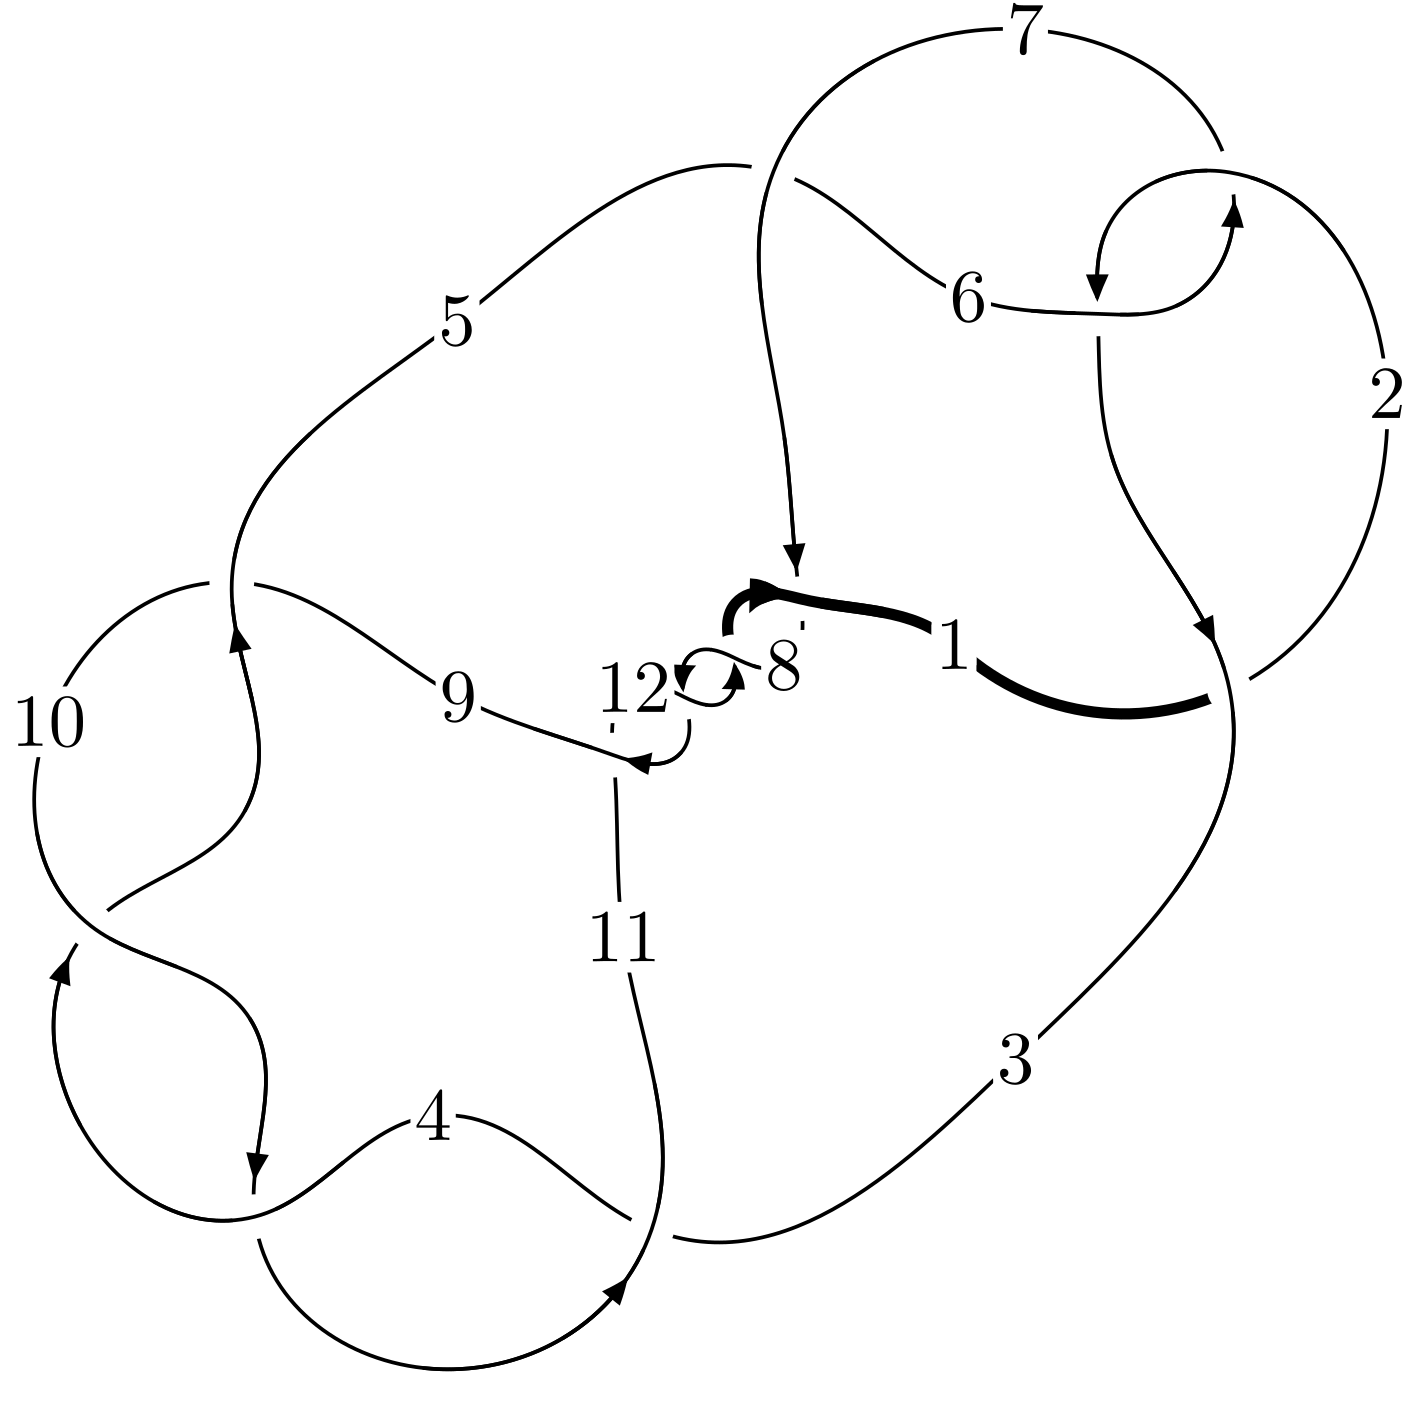
\includegraphics[width=112pt]{../../../GIT/diagram.site/Diagrams/png/1283_12a_0482.png}\\
\ \ \ A knot diagram\footnotemark}&
\allowdisplaybreaks
\textbf{Linearized knot diagam} \\
\cline{2-2}
 &
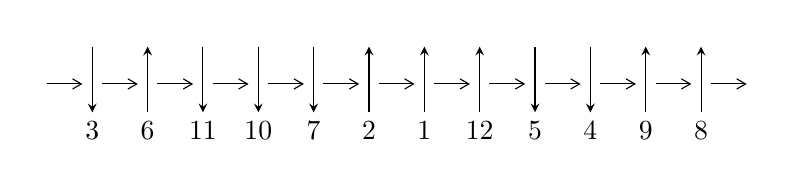
\begin{tikzpicture}[x=20pt, y=17pt]
	% nodes
	\node (C0) at (0, 0) {};
	\node (C1) at (1, 0) {};
	\node (C1U) at (1, +1) {};
	\node (C1D) at (1, -1) {3};

	\node (C2) at (2, 0) {};
	\node (C2U) at (2, +1) {};
	\node (C2D) at (2, -1) {6};

	\node (C3) at (3, 0) {};
	\node (C3U) at (3, +1) {};
	\node (C3D) at (3, -1) {11};

	\node (C4) at (4, 0) {};
	\node (C4U) at (4, +1) {};
	\node (C4D) at (4, -1) {10};

	\node (C5) at (5, 0) {};
	\node (C5U) at (5, +1) {};
	\node (C5D) at (5, -1) {7};

	\node (C6) at (6, 0) {};
	\node (C6U) at (6, +1) {};
	\node (C6D) at (6, -1) {2};

	\node (C7) at (7, 0) {};
	\node (C7U) at (7, +1) {};
	\node (C7D) at (7, -1) {1};

	\node (C8) at (8, 0) {};
	\node (C8U) at (8, +1) {};
	\node (C8D) at (8, -1) {12};

	\node (C9) at (9, 0) {};
	\node (C9U) at (9, +1) {};
	\node (C9D) at (9, -1) {5};

	\node (C10) at (10, 0) {};
	\node (C10U) at (10, +1) {};
	\node (C10D) at (10, -1) {4};

	\node (C11) at (11, 0) {};
	\node (C11U) at (11, +1) {};
	\node (C11D) at (11, -1) {9};

	\node (C12) at (12, 0) {};
	\node (C12U) at (12, +1) {};
	\node (C12D) at (12, -1) {8};
	\node (C13) at (13, 0) {};

	% arrows
	\draw[->,>={angle 60}]
	(C0) edge (C1) (C1) edge (C2) (C2) edge (C3) (C3) edge (C4) (C4) edge (C5) (C5) edge (C6) (C6) edge (C7) (C7) edge (C8) (C8) edge (C9) (C9) edge (C10) (C10) edge (C11) (C11) edge (C12) (C12) edge (C13) ;	\draw[->,>=stealth]
	(C1U) edge (C1D) (C2D) edge (C2U) (C3U) edge (C3D) (C4U) edge (C4D) (C5U) edge (C5D) (C6D) edge (C6U) (C7D) edge (C7U) (C8D) edge (C8U) (C9U) edge (C9D) (C10U) edge (C10D) (C11D) edge (C11U) (C12D) edge (C12U) ;
	\end{tikzpicture} \\
\hhline{~~} \\& 
\textbf{Solving Sequence} \\ \cline{2-2} 
 &
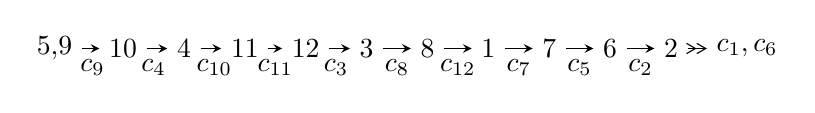
\begin{tikzpicture}[x=22pt, y=7pt]
	% node
	\node (A0) at (-1/8, 0) {5,9};
	\node (A1) at (1, 0) {10};
	\node (A2) at (2, 0) {4};
	\node (A3) at (3, 0) {11};
	\node (A4) at (4, 0) {12};
	\node (A5) at (5, 0) {3};
	\node (A6) at (6, 0) {8};
	\node (A7) at (7, 0) {1};
	\node (A8) at (8, 0) {7};
	\node (A9) at (9, 0) {6};
	\node (A10) at (10, 0) {2};
	\node (C1) at (1/2, -1) {$c_{9}$};
	\node (C2) at (3/2, -1) {$c_{4}$};
	\node (C3) at (5/2, -1) {$c_{10}$};
	\node (C4) at (7/2, -1) {$c_{11}$};
	\node (C5) at (9/2, -1) {$c_{3}$};
	\node (C6) at (11/2, -1) {$c_{8}$};
	\node (C7) at (13/2, -1) {$c_{12}$};
	\node (C8) at (15/2, -1) {$c_{7}$};
	\node (C9) at (17/2, -1) {$c_{5}$};
	\node (C10) at (19/2, -1) {$c_{2}$};
	\node (A11) at (45/4, 0) {$c_{1},c_{6}$};

	% edge
	\draw[->,>=stealth]	
	(A0) edge (A1) (A1) edge (A2) (A2) edge (A3) (A3) edge (A4) (A4) edge (A5) (A5) edge (A6) (A6) edge (A7) (A7) edge (A8) (A8) edge (A9) (A9) edge (A10) ;
	\draw[->>,>={angle 60}]	
	(A10) edge (A11);
\end{tikzpicture} \\ 

\end{tabular} \\

\footnotetext{
The image of knot diagram is generated by the software ``\textbf{Draw programme}" developed by Andrew Bartholomew(\url{http://www.layer8.co.uk/maths/draw/index.htm\#Running-draw}), where we modified some parts for our purpose(\url{https://github.com/CATsTAILs/LinksPainter}).
}\phantom \\ \newline 
\centering \textbf{Ideals for irreducible components\footnotemark of $X_{\text{par}}$} 
 
\begin{align*}
I^u_{1}&=\langle 
u^{46}- u^{45}+\cdots-3 u+1\rangle \\
\\
\end{align*}
\raggedright * 1 irreducible components of $\dim_{\mathbb{C}}=0$, with total 46 representations.\\
\footnotetext{All coefficients of polynomials are rational numbers. But the coefficients are sometimes approximated in decimal forms when there is not enough margin.}
\newpage
\renewcommand{\arraystretch}{1}
\centering \section*{I. $I^u_{1}= \langle u^{46}- u^{45}+\cdots-3 u+1 \rangle$}
\flushleft \textbf{(i) Arc colorings}\\
\begin{tabular}{m{7pt} m{180pt} m{7pt} m{180pt} }
\flushright $a_{5}=$&$\begin{pmatrix}0\\u\end{pmatrix}$ \\
\flushright $a_{9}=$&$\begin{pmatrix}1\\0\end{pmatrix}$ \\
\flushright $a_{10}=$&$\begin{pmatrix}1\\u^2\end{pmatrix}$ \\
\flushright $a_{4}=$&$\begin{pmatrix}u\\u^3+u\end{pmatrix}$ \\
\flushright $a_{11}=$&$\begin{pmatrix}u^2+1\\u^4+2 u^2\end{pmatrix}$ \\
\flushright $a_{12}=$&$\begin{pmatrix}u^4+3 u^2+1\\u^4+2 u^2\end{pmatrix}$ \\
\flushright $a_{3}=$&$\begin{pmatrix}u^3+2 u\\u^5+3 u^3+u\end{pmatrix}$ \\
\flushright $a_{8}=$&$\begin{pmatrix}u^8+5 u^6+7 u^4+2 u^2+1\\u^8+4 u^6+4 u^4\end{pmatrix}$ \\
\flushright $a_{1}=$&$\begin{pmatrix}u^{12}+7 u^{10}+17 u^8+16 u^6+6 u^4+5 u^2+1\\u^{12}+6 u^{10}+12 u^8+8 u^6+u^4+2 u^2\end{pmatrix}$ \\
\flushright $a_{7}=$&$\begin{pmatrix}u^{16}+9 u^{14}+31 u^{12}+50 u^{10}+39 u^8+22 u^6+18 u^4+4 u^2+1\\u^{16}+8 u^{14}+24 u^{12}+32 u^{10}+18 u^8+8 u^6+8 u^4\end{pmatrix}$ \\
\flushright $a_{6}=$&$\begin{pmatrix}- u^{33}-18 u^{31}+\cdots-8 u^3- u\\- u^{33}-17 u^{31}+\cdots-8 u^5+u\end{pmatrix}$ \\
\flushright $a_{2}=$&$\begin{pmatrix}u^{20}+11 u^{18}+\cdots+7 u^2+1\\u^{22}+12 u^{20}+\cdots+8 u^4+3 u^2\end{pmatrix}$\\&\end{tabular}
\flushleft \textbf{(ii) Obstruction class $= -1$}\\~\\
\flushleft \textbf{(iii) Cusp Shapes $= 4 u^{45}-4 u^{44}+\cdots+28 u-6$}\\~\\
\newpage\renewcommand{\arraystretch}{1}
\flushleft \textbf{(iv) u-Polynomials at the component}\newline \\
\begin{tabular}{m{50pt}|m{274pt}}
Crossings & \hspace{64pt}u-Polynomials at each crossing \\
\hline $$\begin{aligned}c_{1},c_{5}\end{aligned}$$&$\begin{aligned}
&u^{46}+17 u^{45}+\cdots+7 u+1
\end{aligned}$\\
\hline $$\begin{aligned}c_{2},c_{6}\end{aligned}$$&$\begin{aligned}
&u^{46}- u^{45}+\cdots- u+1
\end{aligned}$\\
\hline $$\begin{aligned}c_{3},c_{4},c_{9}\\c_{10}\end{aligned}$$&$\begin{aligned}
&u^{46}+u^{45}+\cdots+3 u+1
\end{aligned}$\\
\hline $$\begin{aligned}c_{7},c_{8},c_{11}\\c_{12}\end{aligned}$$&$\begin{aligned}
&u^{46}+5 u^{45}+\cdots+17 u+3
\end{aligned}$\\
\hline
\end{tabular}\\~\\
\newpage\renewcommand{\arraystretch}{1}
\flushleft \textbf{(v) Riley Polynomials at the component}\newline \\
\begin{tabular}{m{50pt}|m{274pt}}
Crossings & \hspace{64pt}Riley Polynomials at each crossing \\
\hline $$\begin{aligned}c_{1},c_{5}\end{aligned}$$&$\begin{aligned}
&y^{46}+25 y^{45}+\cdots+87 y+1
\end{aligned}$\\
\hline $$\begin{aligned}c_{2},c_{6}\end{aligned}$$&$\begin{aligned}
&y^{46}+17 y^{45}+\cdots+7 y+1
\end{aligned}$\\
\hline $$\begin{aligned}c_{3},c_{4},c_{9}\\c_{10}\end{aligned}$$&$\begin{aligned}
&y^{46}+49 y^{45}+\cdots+7 y+1
\end{aligned}$\\
\hline $$\begin{aligned}c_{7},c_{8},c_{11}\\c_{12}\end{aligned}$$&$\begin{aligned}
&y^{46}+53 y^{45}+\cdots+311 y+9
\end{aligned}$\\
\hline
\end{tabular}\\~\\
\newpage\flushleft \textbf{(vi) Complex Volumes and Cusp Shapes}
$$\begin{array}{c|c|c}  
\text{Solutions to }I^u_{1}& \I (\text{vol} + \sqrt{-1}CS) & \text{Cusp shape}\\
 \hline 
\begin{aligned}
u &= \phantom{-}0.664742 + 0.533075 I\end{aligned}
 & -7.89200 - 9.32854 I & -3.38258 + 7.74496 I \\ \hline\begin{aligned}
u &= \phantom{-}0.664742 - 0.533075 I\end{aligned}
 & -7.89200 + 9.32854 I & -3.38258 - 7.74496 I \\ \hline\begin{aligned}
u &= \phantom{-}0.675457 + 0.508562 I\end{aligned}
 & -12.18020 - 2.26977 I & -7.30774 + 2.96998 I \\ \hline\begin{aligned}
u &= \phantom{-}0.675457 - 0.508562 I\end{aligned}
 & -12.18020 + 2.26977 I & -7.30774 - 2.96998 I \\ \hline\begin{aligned}
u &= -0.656275 + 0.523642 I\end{aligned}
 & -6.28780 + 3.84503 I & -1.26707 - 3.22196 I \\ \hline\begin{aligned}
u &= -0.656275 - 0.523642 I\end{aligned}
 & -6.28780 - 3.84503 I & -1.26707 + 3.22196 I \\ \hline\begin{aligned}
u &= \phantom{-}0.676414 + 0.480624 I\end{aligned}
 & -8.04831 + 4.81861 I & -3.86511 - 1.90322 I \\ \hline\begin{aligned}
u &= \phantom{-}0.676414 - 0.480624 I\end{aligned}
 & -8.04831 - 4.81861 I & -3.86511 + 1.90322 I \\ \hline\begin{aligned}
u &= -0.663474 + 0.486446 I\end{aligned}
 & -6.39825 + 0.60169 I & -1.58447 - 2.81268 I \\ \hline\begin{aligned}
u &= -0.663474 - 0.486446 I\end{aligned}
 & -6.39825 - 0.60169 I & -1.58447 + 2.81268 I \\ \hline\begin{aligned}
u &= -0.425584 + 0.580860 I\end{aligned}
 & \phantom{-}0.50678 + 6.63328 I & \phantom{-}0.39470 - 9.97215 I \\ \hline\begin{aligned}
u &= -0.425584 - 0.580860 I\end{aligned}
 & \phantom{-}0.50678 - 6.63328 I & \phantom{-}0.39470 + 9.97215 I \\ \hline\begin{aligned}
u &= \phantom{-}0.370658 + 0.572348 I\end{aligned}
 & \phantom{-}1.34286 - 1.47615 I & \phantom{-}2.76728 + 4.83936 I \\ \hline\begin{aligned}
u &= \phantom{-}0.370658 - 0.572348 I\end{aligned}
 & \phantom{-}1.34286 + 1.47615 I & \phantom{-}2.76728 - 4.83936 I \\ \hline\begin{aligned}
u &= \phantom{-}0.042363 + 0.667552 I\end{aligned}
 & \phantom{-}3.14066 - 2.54958 I & \phantom{-}7.36401 + 3.99068 I \\ \hline\begin{aligned}
u &= \phantom{-}0.042363 - 0.667552 I\end{aligned}
 & \phantom{-}3.14066 + 2.54958 I & \phantom{-}7.36401 - 3.99068 I \\ \hline\begin{aligned}
u &= -0.471349 + 0.440857 I\end{aligned}
 & -3.50342 + 1.63744 I & -7.27018 - 4.90319 I \\ \hline\begin{aligned}
u &= -0.471349 - 0.440857 I\end{aligned}
 & -3.50342 - 1.63744 I & -7.27018 + 4.90319 I \\ \hline\begin{aligned}
u &= -0.04737 + 1.43621 I\end{aligned}
 & \phantom{-}4.81615 - 1.87426 I & \phantom{-0.000000 } 0 \\ \hline\begin{aligned}
u &= -0.04737 - 1.43621 I\end{aligned}
 & \phantom{-}4.81615 + 1.87426 I & \phantom{-0.000000 } 0 \\ \hline\begin{aligned}
u &= -0.487759 + 0.265494 I\end{aligned}
 & -0.43809 - 3.45776 I & -3.80106 + 2.57819 I \\ \hline\begin{aligned}
u &= -0.487759 - 0.265494 I\end{aligned}
 & -0.43809 + 3.45776 I & -3.80106 - 2.57819 I \\ \hline\begin{aligned}
u &= -0.11192 + 1.48925 I\end{aligned}
 & \phantom{-}2.82329 + 3.62355 I & \phantom{-0.000000 } 0 \\ \hline\begin{aligned}
u &= -0.11192 - 1.48925 I\end{aligned}
 & \phantom{-}2.82329 - 3.62355 I & \phantom{-0.000000 } 0 \\ \hline\begin{aligned}
u &= \phantom{-}0.05755 + 1.49977 I\end{aligned}
 & \phantom{-}6.38122 - 1.82382 I & \phantom{-0.000000 } 0 \\ \hline\begin{aligned}
u &= \phantom{-}0.05755 - 1.49977 I\end{aligned}
 & \phantom{-}6.38122 + 1.82382 I & \phantom{-0.000000 } 0 \\ \hline\begin{aligned}
u &= \phantom{-}0.21458 + 1.49604 I\end{aligned}
 & -1.61318 + 1.60482 I & \phantom{-0.000000 } 0 \\ \hline\begin{aligned}
u &= \phantom{-}0.21458 - 1.49604 I\end{aligned}
 & -1.61318 - 1.60482 I & \phantom{-0.000000 } 0 \\ \hline\begin{aligned}
u &= -0.20676 + 1.50200 I\end{aligned}
 & \phantom{-}0.09096 + 3.73634 I & \phantom{-0.000000 } 0 \\ \hline\begin{aligned}
u &= -0.20676 - 1.50200 I\end{aligned}
 & \phantom{-}0.09096 - 3.73634 I & \phantom{-0.000000 } 0\\
 \hline 
 \end{array}$$\newpage$$\begin{array}{c|c|c}  
\text{Solutions to }I^u_{1}& \I (\text{vol} + \sqrt{-1}CS) & \text{Cusp shape}\\
 \hline 
\begin{aligned}
u &= \phantom{-}0.21685 + 1.51393 I\end{aligned}
 & -5.56462 - 5.50465 I & \phantom{-0.000000 } 0 \\ \hline\begin{aligned}
u &= \phantom{-}0.21685 - 1.51393 I\end{aligned}
 & -5.56462 + 5.50465 I & \phantom{-0.000000 } 0 \\ \hline\begin{aligned}
u &= -0.20731 + 1.52424 I\end{aligned}
 & \phantom{-}0.43892 + 6.97774 I & \phantom{-0.000000 } 0 \\ \hline\begin{aligned}
u &= -0.20731 - 1.52424 I\end{aligned}
 & \phantom{-}0.43892 - 6.97774 I & \phantom{-0.000000 } 0 \\ \hline\begin{aligned}
u &= \phantom{-}0.21236 + 1.52855 I\end{aligned}
 & -1.11770 - 12.51940 I & \phantom{-0.000000 } 0 \\ \hline\begin{aligned}
u &= \phantom{-}0.21236 - 1.52855 I\end{aligned}
 & -1.11770 + 12.51940 I & \phantom{-0.000000 } 0 \\ \hline\begin{aligned}
u &= \phantom{-}0.415258 + 0.188192 I\end{aligned}
 & \phantom{-}0.263014 - 1.271440 I & -3.04057 + 3.64034 I \\ \hline\begin{aligned}
u &= \phantom{-}0.415258 - 0.188192 I\end{aligned}
 & \phantom{-}0.263014 + 1.271440 I & -3.04057 - 3.64034 I \\ \hline\begin{aligned}
u &= \phantom{-}0.09628 + 1.54151 I\end{aligned}
 & \phantom{-}8.41953 - 3.11711 I & \phantom{-0.000000 } 0 \\ \hline\begin{aligned}
u &= \phantom{-}0.09628 - 1.54151 I\end{aligned}
 & \phantom{-}8.41953 + 3.11711 I & \phantom{-0.000000 } 0 \\ \hline\begin{aligned}
u &= \phantom{-}0.238736 + 0.384624 I\end{aligned}
 & \phantom{-}0.049172 - 0.835852 I & \phantom{-}1.31520 + 8.15747 I \\ \hline\begin{aligned}
u &= \phantom{-}0.238736 - 0.384624 I\end{aligned}
 & \phantom{-}0.049172 + 0.835852 I & \phantom{-}1.31520 - 8.15747 I \\ \hline\begin{aligned}
u &= -0.11146 + 1.54382 I\end{aligned}
 & \phantom{-}7.60893 + 8.52667 I & \phantom{-0.000000 } 0 \\ \hline\begin{aligned}
u &= -0.11146 - 1.54382 I\end{aligned}
 & \phantom{-}7.60893 - 8.52667 I & \phantom{-0.000000 } 0 \\ \hline\begin{aligned}
u &= \phantom{-}0.00802 + 1.55602 I\end{aligned}
 & \phantom{-}10.58230 - 2.70871 I & \phantom{-0.000000 } 0 \\ \hline\begin{aligned}
u &= \phantom{-}0.00802 - 1.55602 I\end{aligned}
 & \phantom{-}10.58230 + 2.70871 I & \phantom{-0.000000 } 0\\
 \hline 
 \end{array}$$\newpage
\newpage\renewcommand{\arraystretch}{1}
\centering \section*{ II. u-Polynomials}
\begin{tabular}{m{50pt}|m{274pt}}
Crossings & \hspace{64pt}u-Polynomials at each crossing \\
\hline $$\begin{aligned}c_{1},c_{5}\end{aligned}$$&$\begin{aligned}
&u^{46}+17 u^{45}+\cdots+7 u+1
\end{aligned}$\\
\hline $$\begin{aligned}c_{2},c_{6}\end{aligned}$$&$\begin{aligned}
&u^{46}- u^{45}+\cdots- u+1
\end{aligned}$\\
\hline $$\begin{aligned}c_{3},c_{4},c_{9}\\c_{10}\end{aligned}$$&$\begin{aligned}
&u^{46}+u^{45}+\cdots+3 u+1
\end{aligned}$\\
\hline $$\begin{aligned}c_{7},c_{8},c_{11}\\c_{12}\end{aligned}$$&$\begin{aligned}
&u^{46}+5 u^{45}+\cdots+17 u+3
\end{aligned}$\\
\hline
\end{tabular}\newpage\renewcommand{\arraystretch}{1}
\centering \section*{ III. Riley Polynomials}
\begin{tabular}{m{50pt}|m{274pt}}
Crossings & \hspace{64pt}Riley Polynomials at each crossing \\
\hline $$\begin{aligned}c_{1},c_{5}\end{aligned}$$&$\begin{aligned}
&y^{46}+25 y^{45}+\cdots+87 y+1
\end{aligned}$\\
\hline $$\begin{aligned}c_{2},c_{6}\end{aligned}$$&$\begin{aligned}
&y^{46}+17 y^{45}+\cdots+7 y+1
\end{aligned}$\\
\hline $$\begin{aligned}c_{3},c_{4},c_{9}\\c_{10}\end{aligned}$$&$\begin{aligned}
&y^{46}+49 y^{45}+\cdots+7 y+1
\end{aligned}$\\
\hline $$\begin{aligned}c_{7},c_{8},c_{11}\\c_{12}\end{aligned}$$&$\begin{aligned}
&y^{46}+53 y^{45}+\cdots+311 y+9
\end{aligned}$\\
\hline
\end{tabular}
\vskip 2pc
\end{document}